\subsection{The Bin Packing Problem (bin\_pack\_func.py)} \label{sbs:binpack}

The solution of the bin packing problem determines where, amongst $m$ ``bins'', to place $n$ ``items'' of various ``sizes'' in a way that (in this case study) minimises the wasted ``capacity'' of the bins. Each product $j=1, \ldots, n$ has a size $s_j$ and each bin has capacity $C$. Extensions of this problem arise often in \ac{MILP} in problems including network design and rostering.

The \ac{MILP} formulation of the bin packing problem is straightforward. The decision variables are
\begin{align*}
x_{ij} &= \begin{cases} 1 & \text{if item $j$ is placed in bin $i$} \\
0 & \text{otherwise} \end{cases} \\
y_i &= \begin{cases} 1 & \text{if a facility is located at location $i$} \\
0 & \text{otherwise} \end{cases} \\
w_i &= \text{ ``wasted'' capacity at location $i$}
\end{align*}
and the formulation is
\[
\begin{array}{rr@{\ }ll}
       \min & \displaystyle \sum_{i=1}^m w_i \\
\text{s.t.} & \displaystyle \sum_{i=1}^m x_{ij}           & = 1, j = 1, \ldots, n      & \text{ (each product produced)} \\
            & \displaystyle \sum_{j=1}^n r_j x_{ij} + w_i & = C y_i, i = 1, \ldots, m  & \text{ (aggregate capacity at location $i$)} \\
            & \multicolumn{2}{l}{x_{ij} \leq y_i, i = 1, \ldots, m, j = 1, \ldots, n}  & \text{ (disaggregate capacity at location $i$)} \\[6pt]
            & \multicolumn{3}{l}{x_{ij} \in \{ 0, 1\}, w_i \geq 0, y_i \in \{0, 1\}, i = 1, \ldots, m, j = 1, \ldots, n}
\end{array}
\]

Note that the disaggregate capacity constraints are not necessary for defining the solution, but tighten the \ac{MILP} formulation ( i.e., remove factional solutions from the solution space). Using PuLP we can easily define this \ac{MILP} problemm in Dippy. The entire input file is given below with a summary for each fragment.

\begin{enumerate}
\item Load PuLP and Dippy;
\lstinputlisting[linerange=3-20]{../../examples/Dippy/bpp/bin_pack_func.py}

\item Get the problem data from another file. This determines $j=1, \ldots, n$, $i = 1, \ldots, m$, $r_j, j = 1, \ldots, n$ and $C$;
\lstinputlisting[firstnumber=9,linerange=9-10]{../../examples/Dippy/bpp/bin_pack_func.py}
For {\tt facility\_ex1.py} $n = 5, m = 5, r = (7, 5, 3, 2, 2)^\top$ and $C = 8$.

\item Define the \ac{MILP} problem and the problem variables;
\lstinputlisting[firstnumber=15,linerange=15-24]{../../examples/Dippy/bpp/bin_pack_func.py}

\item Define the objective function;
\lstinputlisting[firstnumber=26,linerange=26-27]{../../examples/Dippy/bpp/bin_pack_func.py}

\item Define the constraints; \lstinputlisting[firstnumber=29,linerange=29-42]{../../examples/Dippy/bpp/bin_pack_func.py}

\item Solve the \ac{MILP} problem using \ac{DIP} using default options except for a user-defined zero tolerance and then display the solution;
\lstinputlisting[firstnumber=235,linerange=235-244]{../../examples/Dippy/bpp/bin_pack_func.py}
\end{enumerate}
Running the preceding Python codes takes 1.17s of CPU time, creates a tree with 375 nodes and gives the following output
\begin{verbatim}
Location  1  produces  [1]
Location  4  produces  [4, 5]
Location  5  produces  [2, 3]
\end{verbatim}

Note that \ac{DIP} uses cuts from the \ac{CGL} \cite{coin_or} by default. We can turn all cuts off by setting the {\tt generateCuts} flag to 0 and turn \ac{CGL} cuts off by setting the {\tt CutCGL} flag to 0. We will use these settings to explore the effect of user-defined cuts in \scnref{scn:cuts}.

We will use the Bin Packing Problem to demonstrate the implementation of customised branching rules, custom cuts, heuristics, and a column generation algorithm.

The solution of the problem determines which, of $m$ bins, to use and also places $n$ items of various sizes into the bins in a way that (in this version) minimises the wasted capacity of the bins.
Each item $j=1, \ldots, n$ has a size $s_j$ and each bin has capacity $C$.
Extensions of this problem arise often in \ac{MILP} in problems including network design and rostering.

The \ac{MILP} formulation of the bin packing problem is straightforward.
The decision variables are
\begin{align*}
x_{ij} &= \begin{cases} 1 & \text{if item $j$ is placed in bin $i$} \\
0 & \text{otherwise} \end{cases} \\
y_i &= \begin{cases} 1 & \text{if bin $i$ is used} \\
0 & \text{otherwise} \end{cases} \\
w_i &= \text{ ``wasted'' capacity in bin $i$}
\end{align*}
and the formulation is
\[
\begin{array}{rr@{\ }ll}
       \min & \displaystyle \sum_{i=1}^m w_i \\
\text{s.t.} & \displaystyle \sum_{i=1}^m x_{ij}           & = 1, j = 1, \ldots, n      & \text{ (each item packed)} \\
            & \displaystyle \sum_{j=1}^n s_j x_{ij} + w_i & = C y_i, i = 1, \ldots, m  & \text{ (aggregate packing for bin $i$)} \\
            & \multicolumn{2}{l}{x_{ij} \leq y_i, i = 1, \ldots, m, j = 1, \ldots, n}  & \text{ (individual packing for bin $i$)} \\[6pt]
            & \multicolumn{3}{l}{x_{ij} \in \{ 0, 1\}, w_i \geq 0, y_i \in \{0, 1\}, i = 1, \ldots, m, j = 1, \ldots, n}
\end{array}
\]

Note that the constraints for the individual packing in a bin are not necessary for defining the solution, but tighten the \ac{MILP} formulation by removing fractional solutions from the solution space. Before looking at the advanced techniques that can be easily implemented using Dippy, we will examine how to formulate the bin packing problem in PuLP and Dippy.

\subsection{Formulating the Bin Packing Problem} \label{sbs:formulate}

Before formulating we need to include the PuLP and Dippy modules into Python
\lstinputlisting[firstnumber=3,linerange=3-21]{../../examples/Dippy/bpp/bin_pack_func.py}
and define a class to hold a bin packing problem's data
\lstinputlisting[firstnumber=25,linerange=25-31]{../../examples/Dippy/bpp/bin_pack_func.py}

The \lstinline{formulate} function is defined with a bin packing problem object as input and creates a \lstinline{DipProblem} (with some display options defined)
\lstinputlisting[firstnumber=33,linerange=33-38]{../../examples/Dippy/bpp/bin_pack_func.py}

Then, using the bin packing problem object's data (i.e., the data defined within \lstinline{bpp}), the decision variables
\lstinputlisting[firstnumber=40,linerange=40-45]{../../examples/Dippy/bpp/bin_pack_func.py}
objective function
\lstinputlisting[firstnumber=47,linerange=47-47]{../../examples/Dippy/bpp/bin_pack_func.py}
\newpage
and constraints are defined
\lstinputlisting[firstnumber=49,linerange=49-59]{../../examples/Dippy/bpp/bin_pack_func.py}

Finally, the bin packing problem object and the decision variables are all ``embedded'' within the \lstinline{DipProblem} object, \lstinline{prob}, and this object is returned (note that the objective function and constraints could also be similarly embedded)
\lstinputlisting[firstnumber=64,linerange=64-71]{../../examples/Dippy/bpp/bin_pack_func.py}

In order to solve the bin packing problem, only the \lstinline{DipProblem} object, \lstinline{prob}, is required (note that no \lstinline{dippyOpts} are specified, so the Dippy defaults are used)
\lstinputlisting[firstnumber=73,linerange={100-101,108-108,115-122}]{../../examples/Dippy/bpp/bin_pack_func.py}

To solve an instance of the bin packing problem, the data needs to be specified and then the problem formulated and solved
\lstinputlisting[firstnumber=3,linerange=3-11]{../../examples/Dippy/bpp/bin_pack_instance.py}
\lstinputlisting[firstnumber=13,linerange=13-21]{../../examples/Dippy/bpp/bin_pack_instance.py}

Solving this bin packing problem instance in Dippy gives the branch-and-bound tree shown in figure \ref{fig:bpp_tree1} (note thet the integer solution found -- indicated in blue \lstinline{S: 5.0} -- bounds all other nodes in the tree) with the final solution packing items 1 and 2 into bin 0 (for a waste of 1), items 3 and 5 into bin 1 (for a waste of 3) and item 4 into bin 3 (for a waste of 1).
\begin{figure}[htp]
\begin{center}
%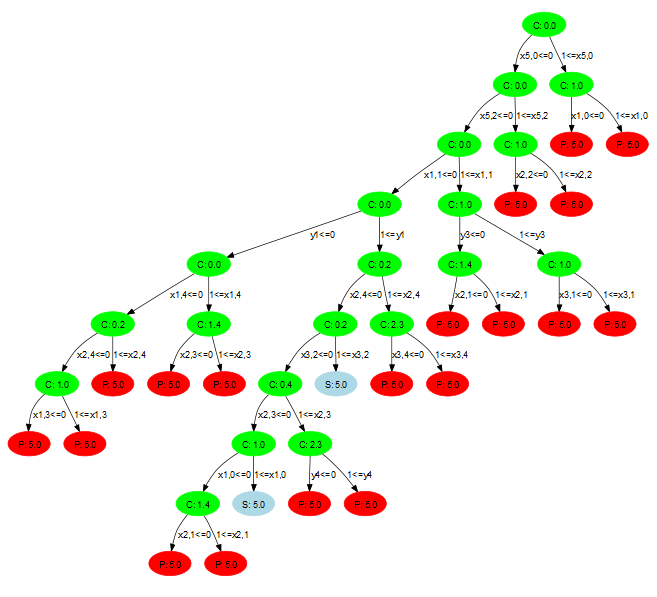
\includegraphics[bb=0 0 815 496,scale=0.50]{img/bpp_tree1.png}
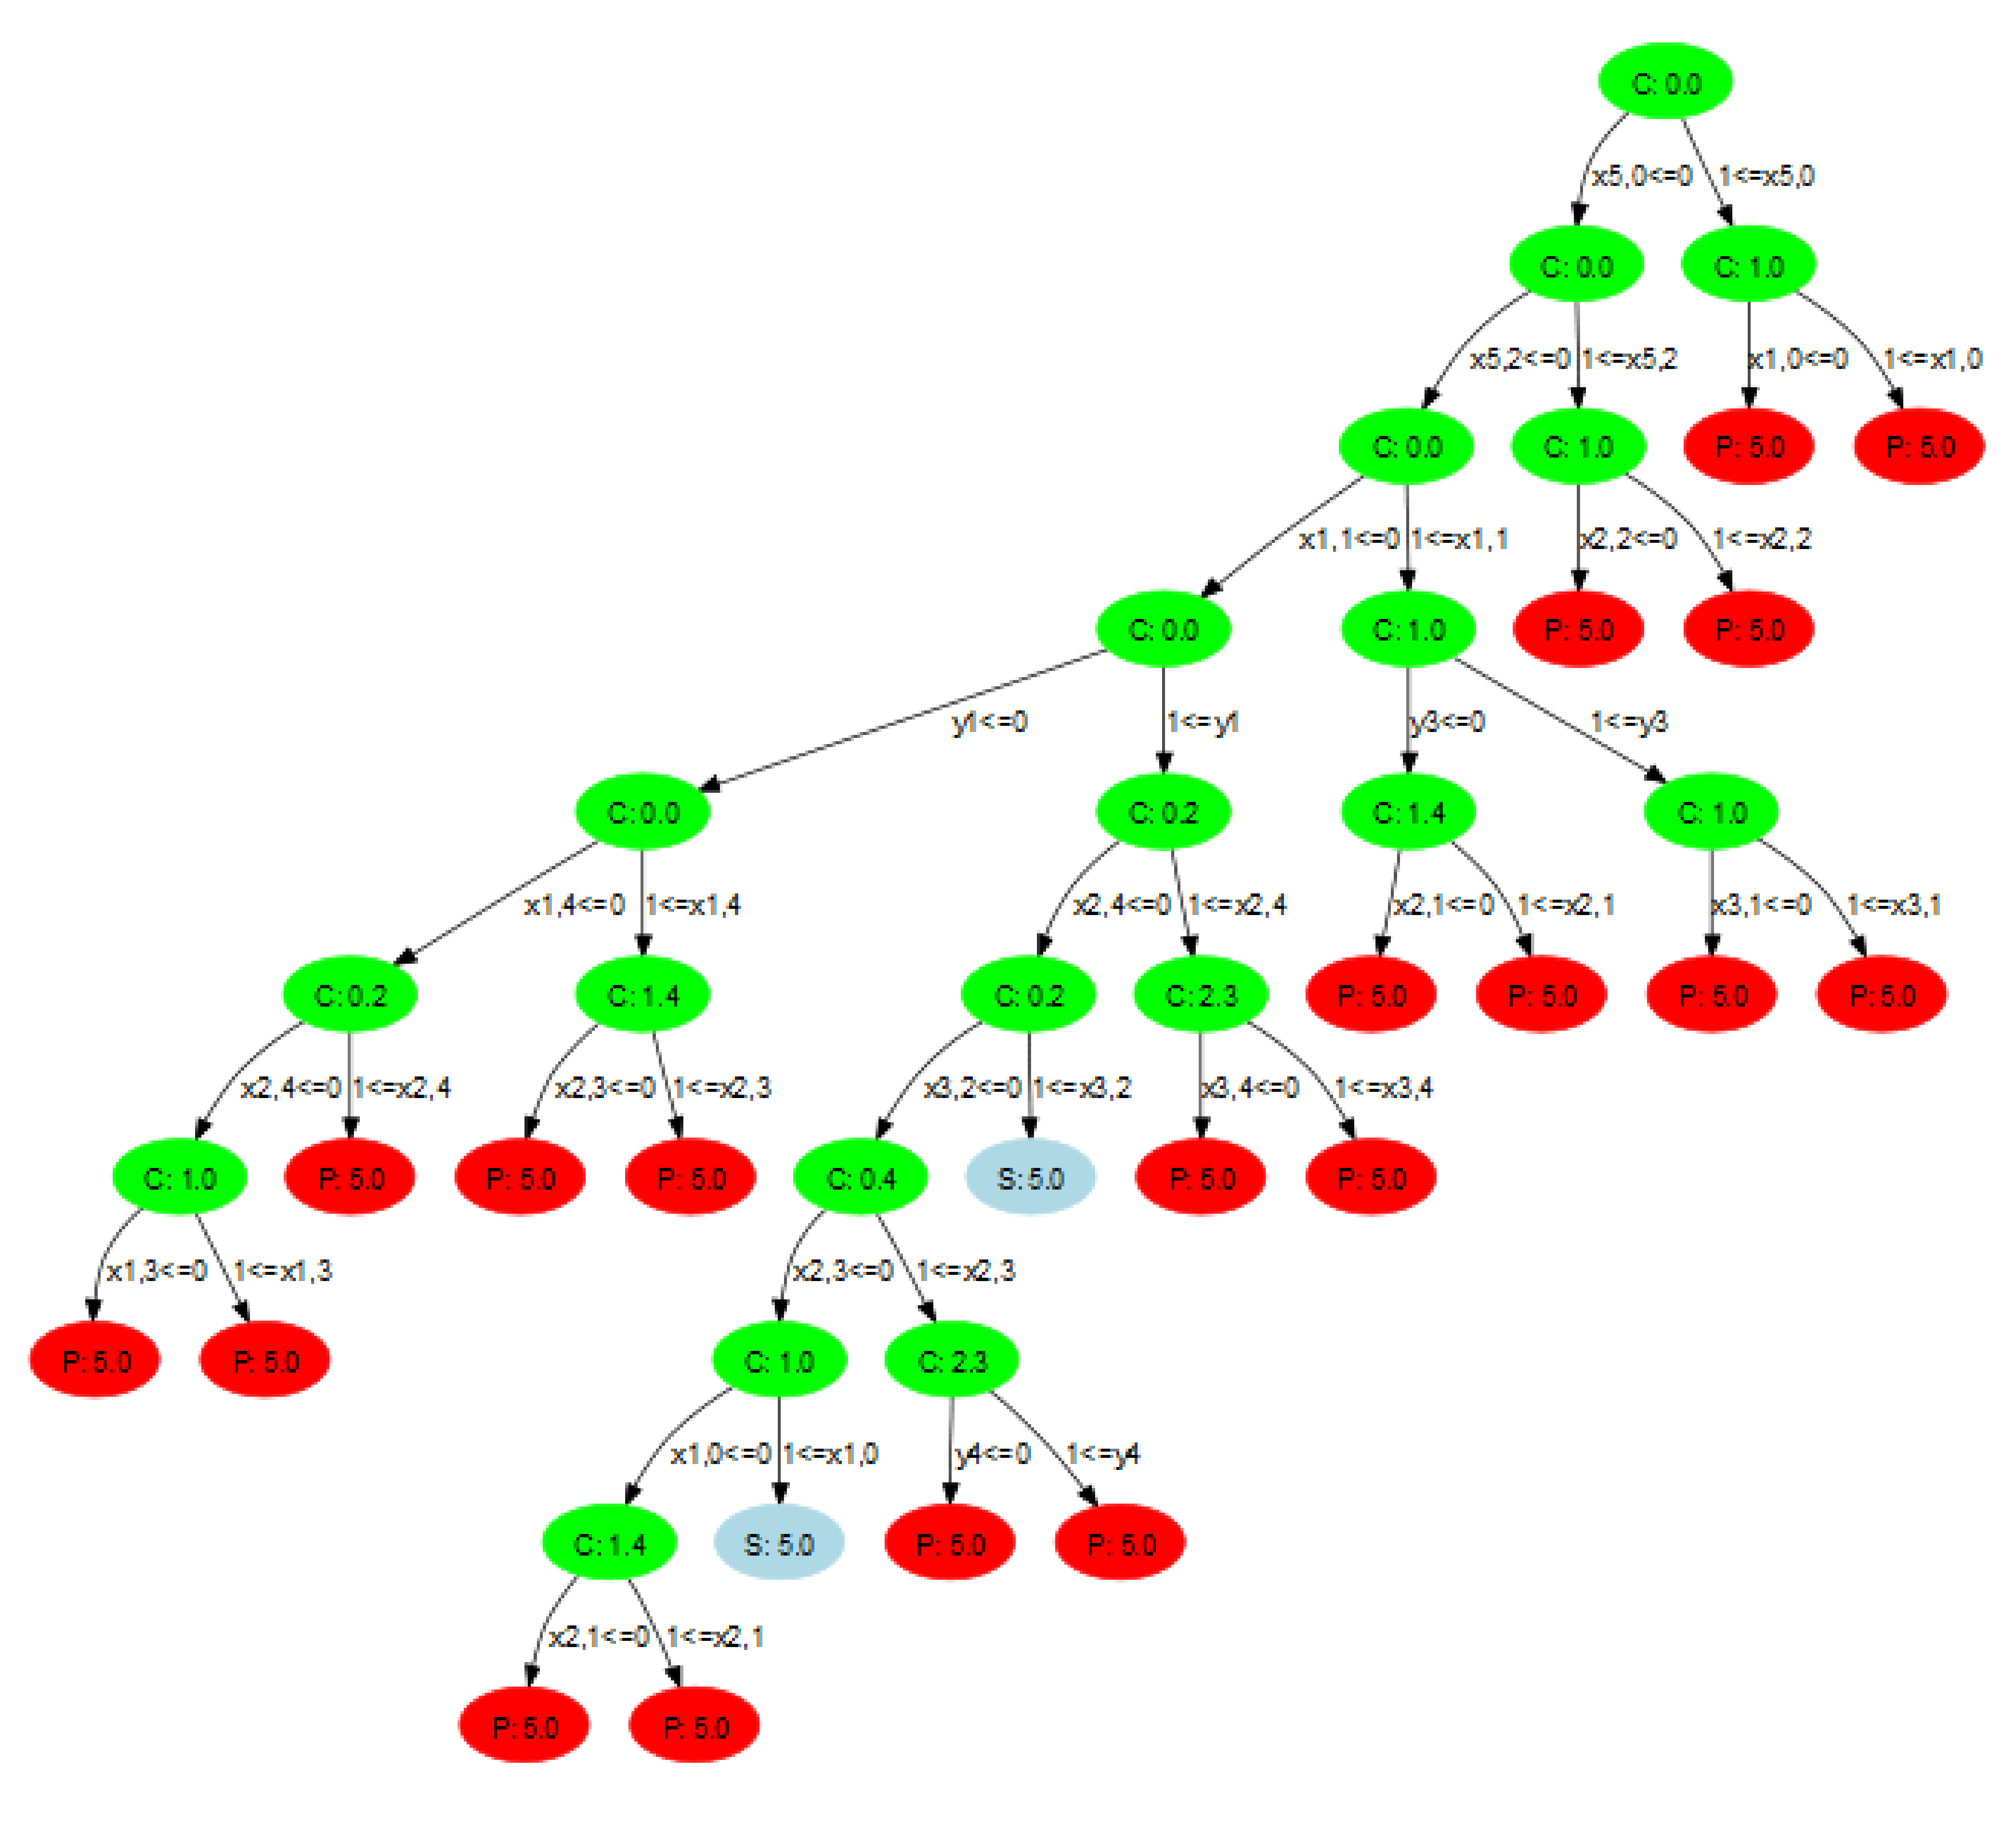
\includegraphics[scale=0.16]{img/bpp_tree1.eps}
\end{center}
\caption{Branch-and-bound tree for bin packing problem instance.} \label{fig:bpp_tree1}
\end{figure}
